\chapter{Combinational circuits}
\label{ch:comb}

Chapter 8 gave us the alphabet; this chapter builds the words.
Every useful digital circuit reduces to a handful of combinational
\emph{building blocks}\index{combinational logic} — multiplexers and
decoders route, adders and comparators compute, and all of them together
form the ALU at the heart of a CPU. After this chapter you will be able
to build a mux from gates and from \texttt{assign}, explain why a
ripple-carry adder is slow, decode a seven-segment display, and count
the speed/area trade in gate delays.

% from-zero:begin
\begin{rulebox}[Before you start]
Chapter~8 (Boolean algebra). \emph{Recap:} \emph{combinational} means the output depends only on the present inputs --- no memory.
\end{rulebox}
\begin{wins}[After this chapter you can]
\begin{itemize}
\item build a multiplexer and a decoder from gates;
\item build a ripple-carry adder and count its delay;
\item design a seven-segment decoder;
\item explain how these blocks become an ALU.
\end{itemize}
\end{wins}
\begin{principle}[How to think about this]
Combinational design is like building with plumbing: signals flow through, and the output simply reflects the input after a delay. The delay matters: a long chain of gates is slow, which is why the structure of an adder affects how fast a computer can run.
\end{principle}
% from-zero:end

\section{Multiplexers and decoders: the two routers}
\label{sec:routers}

A \emph{multiplexer}\index{multiplexer} (mux) selects one of $2^n$ inputs
according to $n$ select lines: $y = d_{s}$. Built from gates it is a
2-level sum-of-products — a decoder of $s$ feeding ANDs whose outputs
OR together. Its dual, the \emph{decoder}\index{decoder}, spreads one
enable into $2^n$ mutually-exclusive lines: $y_i = e \cdot [s=i]$.
Together they are the routers of combinational logic — mux chooses a
path, decoder chooses a destination.

\begin{exercise}[easy]
Write the sum-of-products for a 2:1 mux in terms of $s, d_0, d_1$; then
show it collapses to $\bar s d_0 + s d_1$.
\end{exercise}

\begin{figure}[htbp]
\centering
% 4:1 mux tree from three 2:1 muxes (rectangle muxes for clarity)
\begin{tikzpicture}[font=\footnotesize,
  mux/.style={draw, minimum width=1.4cm, minimum height=1.0cm}]
\node[mux] (m1) at (0,1.2) {};
\node[mux] (m2) at (0,-0.4) {};
\node[mux] (m3) at (3,0.4) {};
\draw[->] (-2.0,1.6) node[left] {$d_0$} -- (m1.west |- -0,1.6);
\draw[->] (-2.0,0.8) node[left] {$d_1$} -- (m1.west |- -0,0.8);
\draw[->] (-2.0,0.0) node[left] {$d_2$} -- (m2.west |- -0,0.0);
\draw[->] (-2.0,-0.8) node[left] {$d_3$} -- (m2.west |- -0,-0.8);
\node[right, font=\scriptsize] at (m1.east) {};
\draw[->] (m1.east) -- ++(0.6,0) |- ($(m3.west)+(0,0.25)$);
\draw[->] (m2.east) -- ++(0.6,0) |- ($(m3.west)+(0,-0.25)$);
\node[above, font=\scriptsize] at ($(m3.west)+(0,0.25)$) {};
\draw[->] (0,-1.7) node[below] {$s_0$} -- (0,-0.9) |- (m1.south);
\draw[->] (m2.south) ++(0,-0.6) -- (m2.south);
\draw[->] (3,-1.4) node[below] {$s_1$} -- (m3.south);
\draw[->] (m3.east) -- ++(0.5,0) node[right] {$y$};
\end{tikzpicture}

\caption{A 4:1 mux as a tree of three 2:1 muxes. Notice the select fanout:
$s_0$ picks inside the leaves, $s_1$ picks between them — the same
address-decoding pattern repeats all the way up to memory chips.}
\label{fig:muxtree}
\end{figure}

\section{Worked example 1: a 4:1 mux, gates then \texttt{assign}}
\label{sec:we-mux}

\textbf{Strategy.} Build it twice — once as a gate tree so the cost is
visible, once as a one-line \texttt{assign} so the intent is — and
convince ourselves the synthesizer sees them as the same circuit.

\textbf{Solution.} As gates, Figure~\ref{fig:muxtree}: three 2:1 muxes,
2 levels of logic, $s_0$ at the leaves, $s_1$ at the root. In Verilog it
collapses to a single selection:
\begin{lstlisting}[caption={The same 4:1 mux as one \texttt{assign}
--- read-only here; toolchain formalised in ch11.},abovecaptionskip=0pt]
assign y = s1 ? (s0 ? d3 : d2) : (s0 ? d1 : d0);
\end{lstlisting}
The ternary nest reads exactly like the tree: top-level \texttt{s1?}
chooses a branch, each \texttt{s0?} chooses a leaf. Synthesis maps both
descriptions to the same lookup table; the \texttt{assign} version wins
because it says \emph{what} and leaves the \emph{how} to the tool.

\section{Adders: half, full, and ripple-carry}
\label{sec:adders}

A \emph{half adder}\index{half adder} adds two bits: $s=a\oplus b$,
$c=ab$ — an XOR and an AND. A \emph{full adder}\index{full adder} adds
three (two operands plus carry-in):
$s=a\oplus b\oplus c_{in}$ and $c_{out}=ab+c_{in}(a\oplus b)$ — two XORs,
two ANDs, an OR (Figure~\ref{fig:fulladder}).

\begin{figure}[htbp]
\centering
% full adder gate map: sum = a^b^cin ; cout = ab + cin(a^b)
\begin{circuitikz}[american, scale=0.75, transform shape, font=\footnotesize]
\node[american xor port] (x1) at (0,2.0) {};
\node[american xor port] (x2) at (2.4,1.7) {};
\node[american and port] (a1) at (0.6,0.0) {};
\node[american and port] (a2) at (2.4,0.4) {};
\node[american or port]  (o1) at (4.4,0.6) {};
\draw (x1.in 1) to[short,-o] ++(-0.9,0) node[left] {$a$};
\draw (x1.in 2) to[short,-o] ++(-0.9,0) node[left] {$b$};
\draw (x1.out) -| (x2.in 1);
\draw (x2.in 2) to[short,-o] ++(-2.6,0) node[left] {$c_{in}$};
\draw (x2.out) to[short,-o] ++(0.5,0) node[right] {sum};
\draw (a1.in 1) to[short,-o] ++(-1.5,0) node[left] {$a$};
\draw (a1.in 2) to[short,-o] ++(-1.5,0) node[left] {$b$};
\draw (a1.out) -| (o1.in 2);
\draw (x1.out) ++(0.4,0) -- ++(0,-0.9) -| (a2.in 1);
\draw (x2.in 2) ++(-0.4,0) -- ++(0,-1.0) -| (a2.in 2);
\draw (a2.out) -| (o1.in 1);
\draw (o1.out) to[short,-o] ++(0.4,0) node[right] {$c_{out}$};
\end{circuitikz}

\caption{Full-adder gate map. Notice the shared $a\oplus b$ feeding both
the sum XOR and the carry AND — reusing a partial result is the whole
trick, and why the gate count is 5 not 7.}
\label{fig:fulladder}
\end{figure}

\begin{lstlisting}[caption={\ttfamily code/ch09\_full\_adder.v --- the
cell the ripple reuses.},label={lst:fa},abovecaptionskip=0pt]
module full_adder(a, b, cin, sum, cout);
  input  a, b, cin;
  output sum, cout;
  assign sum  = a ^ b ^ cin;
  assign cout = (a & b) | (cin & (a ^ b));
endmodule
\end{lstlisting}

Chaining four cells gives the \emph{ripple-carry
adder}\index{ripple-carry adder} of Figure~\ref{fig:ripple}: each carry
must \emph{settle} before the next full adder can even start — the carry
\emph{ripples} through.

\begin{figure}[htbp]
\centering
% 4-bit ripple carry annotated with propagation delay
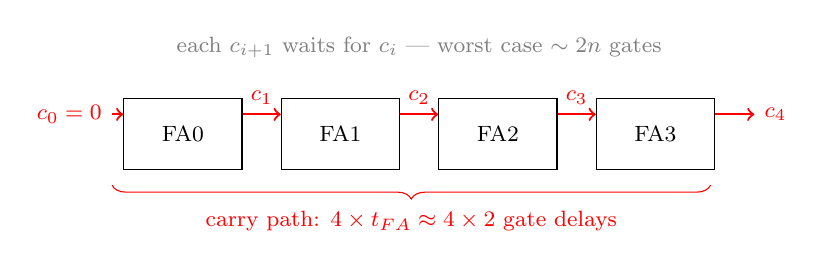
\begin{tikzpicture}[font=\footnotesize, cell/.style={draw, minimum width=1.5cm, minimum height=0.9cm}]
\node[cell] (f0) at (0,0) {FA0};
\node[cell] (f1) at (2,0) {FA1};
\node[cell] (f2) at (4,0) {FA2};
\node[cell] (f3) at (6,0) {FA3};
\draw[->, red, thick] (-0.9,0.25) node[left] {$c_0=0$} -- (f0.west|-0,0.25);
\draw[->, red, thick] (f0.east|-0,0.25) -- node[above] {$c_1$} (f1.west|-0,0.25);
\draw[->, red, thick] (f1.east|-0,0.25) -- node[above] {$c_2$} (f2.west|-0,0.25);
\draw[->, red, thick] (f2.east|-0,0.25) -- node[above] {$c_3$} (f3.west|-0,0.25);
\draw[->, red, thick] (f3.east|-0,0.25) -- ++(0.5,0) node[right] {$c_4$};
\draw[red, decorate, decoration={brace, mirror, amplitude=5pt}] (-0.9,-0.65) -- (6.7,-0.65)
  node[midway, below=6pt] {carry path: $4\times t_{FA}\approx 4\times 2$ gate delays};
\node[gray] at (3,1.1) {each $c_{i+1}$ waits for $c_i$ — worst case $\sim2n$ gates};
\end{tikzpicture}

\caption{The ripple carry chain. Notice what is \emph{not} parallel:
$c_4$ is a function of every bit upstream, so the worst-case delay grows
with $n$, not with the answer's size.}
\label{fig:ripple}
\end{figure}

\begin{lstlisting}[caption={\ttfamily code/ch09\_adder4.v + its
testbench --- the 4-cell chain, exercised.},label={lst:adder4},abovecaptionskip=0pt]
module adder4(a, b, sum, cout);
  input  [3:0] a, b;
  output [3:0] sum;
  output       cout;
  wire [2:0]   c;
  full_adder fa0(.a(a[0]), .b(b[0]), .cin(1'b0),  .sum(sum[0]), .cout(c[0]));
  full_adder fa1(.a(a[1]), .b(b[1]), .cin(c[0]),  .sum(sum[1]), .cout(c[1]));
  full_adder fa2(.a(a[2]), .b(b[2]), .cin(c[1]),  .sum(sum[2]), .cout(c[2]));
  full_adder fa3(.a(a[3]), .b(b[3]), .cin(c[2]),  .sum(sum[3]), .cout(cout));
endmodule
\end{lstlisting}

\begin{lstlisting}[caption={Last rows of the real \texttt{vvp} output ---
carry out asserted at 15+5, 15+10, 15+15.},abovecaptionskip=0pt]
 a +  b = (cout,sum)
15 + 10 = (1, 9)
15 + 15 = (1,14)
ch09_adder4_tb.v:16: $finish called at 64000 (1ps)
\end{lstlisting}

\section{Worked example 2: counting the delay}
\label{sec:we-delay}

\textbf{Strategy.} Estimate the ripple's worst-case delay honestly, then
compare a 2-level (sum-of-products) alternative — and see why the trade
is speed \emph{vs} area, not free lunch.

\textbf{Solution.} Each full adder's carry-out is 2 gate-delays after its
carry-in settles (XOR then AND-OR). For a 4-bit ripple the carry walks
$4\times 2=8$ levels; for $n$ bits, $\approx 2n$. The alternative —
compute carry directly as a 2-level function of all $2n$ inputs — needs
$2^n$ product terms per carry: $n=8$ needs 256 AND gates per carry
versus 8 FAs. Figure~\ref{fig:adderblock} sketches the real compromise
(carry-lookahead, built properly later): more logic in exchange for a
bounded $\sim$4-level path. The lesson is the \emph{trade itself}: in
combinational design there is almost always a faster circuit if you are
willing to pay for it in gates.

\begin{figure}[htbp]
\centering
% adder block diagram, CLA teaser
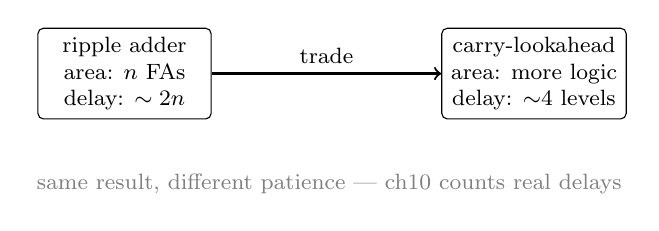
\begin{tikzpicture}[font=\footnotesize, box/.style={draw, rounded corners=2pt, minimum width=2.2cm, minimum height=1.0cm, align=center}]
\node[box] (rc) at (0,0) {ripple adder\\ area: $n$ FAs\\ delay: $\sim2n$};
\node[box] (cla) at (5.2,0) {carry-lookahead\\ area: more logic\\ delay: $\sim$4 levels};
\draw[->, thick] (rc) -- (cla) node[midway, above] {trade};
\node[gray] at (2.6,-1.4) {same result, different patience — ch10 counts real delays};
\end{tikzpicture}

\caption{Speed-vs-area in one picture. Notice both blocks produce the
same sum — only the \emph{path length} to it differs.}
\label{fig:adderblock}
\end{figure}

\begin{exercise}[medium]
An 8-bit ripple adder is roughly $2\times$ a 4-bit's delay and $8\times$
the two-level carry logic's area. Write the delay for $n=16$ and the
product-term count for the 2-level $c_{16}$ alternative.
\end{exercise}

\section{Comparators, encoders, priority}
\label{sec:priority}

A \emph{comparator}\index{comparator (digital)} is a subtractor that
keeps only the sign: equality is an XNOR tree, magnitude falls out of
the borrow chain. An \emph{encoder}\index{encoder} runs a decoder
backwards — $2^n$ lines in, $n$ bits out — and a \emph{priority
encoder} resolves ties by position, which is exactly what an interrupt
controller does: \texttt{casez} with wildcard rows, don't-cares marking
``lower priority does not matter.''

\textbf{Don't-cares}\index{don't-care} are a contract, not an omission:
writing \texttt{x} on impossible inputs lets the minimizer pick the
cheaper neighbor — but only for inputs the rest of the system truly
never produces.

\section{Worked example 3: seven-segment decoder}
\label{sec:we-seg7}

\textbf{Strategy.} A digit $\to$ 7 segments is just 7 Boolean functions
of 4 inputs. Write the truth table once (rows 10--15 as don't-cares),
minimize each segment, then let a \texttt{case} statement say it plainly
and the simulator print the check.

\textbf{Solution.} The segment map is Figure~\ref{fig:seg7map}; the
decoder and its \texttt{case}:

\begin{lstlisting}[caption={\ttfamily code/ch09\_seg7.v --- BCD to
cathodes \texttt{\{a,b,c,d,e,f,g\}}.},label={lst:seg7},abovecaptionskip=0pt]
module seg7(d, seg);
  input  [3:0] d;
  output reg [6:0] seg;
  always @(*) begin
    case (d)
      4'd0: seg = 7'b1111110;
      4'd1: seg = 7'b0110000;
      4'd2: seg = 7'b1101101;
      4'd3: seg = 7'b1111001;
      4'd4: seg = 7'b0110011;
      4'd5: seg = 7'b1011011;
      4'd6: seg = 7'b1011111;
      4'd7: seg = 7'b1110000;
      4'd8: seg = 7'b1111111;
      4'd9: seg = 7'b1111011;
      default: seg = 7'b0000000;
    endcase
  end
endmodule
\end{lstlisting}

\begin{lstlisting}[caption={Real truth-dump of
\texttt{ch09\_seg7\_tb.v} --- digits 0--9 plus the don't-care rows.},abovecaptionskip=0pt]
 d | abcdefg
---+--------
 0 | 1111110
 1 | 0110000
 2 | 1101101
 3 | 1111001
 4 | 0110011
 5 | 1011011
 6 | 1011111
 7 | 1110000
 8 | 1111111
 9 | 1111011
10 | 0000000
...
15 | 0000000
\end{lstlisting}

The \texttt{default} is the don't-care policy made concrete: rows the
driver never produces get \texttt{x} on paper and \texttt{0000000} here —
the display dark rather than arbitrary.

\begin{figure}[htbp]
\centering
% seven-segment letter map + seg-e example cells
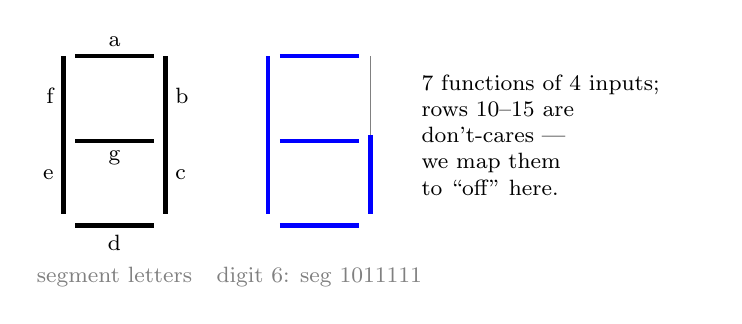
\begin{tikzpicture}[font=\footnotesize]
% segment map
\draw[ultra thick] (0,2) -- (1,2); \node[above] at (0.5,2) {a};
\draw[ultra thick] (1.15,1) -- (1.15,2); \node[right] at (1.15,1.5) {b};
\draw[ultra thick] (1.15,0) -- (1.15,1); \node[right] at (1.15,0.5) {c};
\draw[ultra thick] (0,-0.15) -- (1,-0.15); \node[below] at (0.5,-0.15) {d};
\draw[ultra thick] (-0.15,0) -- (-0.15,1); \node[left] at (-0.15,0.5) {e};
\draw[ultra thick] (-0.15,1) -- (-0.15,2); \node[left] at (-0.15,1.5) {f};
\draw[ultra thick] (0,0.92) -- (1,0.92); \node[below] at (0.5,0.92) {g};
\node[gray] at (0.5,-0.8) {segment letters};
% lit shape for digit 6 (a f g e d c on, b off)
\begin{scope}[xshift=2.6cm]
\draw[ultra thick, blue] (0,2) -- (1,2);
\draw[thin, gray] (1.15,1) -- (1.15,2);
\draw[ultra thick, blue] (1.15,0) -- (1.15,1);
\draw[ultra thick, blue] (0,-0.15) -- (1,-0.15);
\draw[ultra thick, blue] (-0.15,0) -- (-0.15,1);
\draw[ultra thick, blue] (-0.15,1) -- (-0.15,2);
\draw[ultra thick, blue] (0,0.92) -- (1,0.92);
\node[gray] at (0.5,-0.8) {digit 6: seg 1011111};
\end{scope}
% don't-care policy note
\begin{scope}[xshift=6.2cm]
\node[align=left, text width=3.6cm] at (0,1.0)
 {7 functions of 4 inputs;\\ rows 10--15 are\\ don't-cares —\\ we map them\\ to ``off'' here.};
\end{scope}
\end{tikzpicture}

\caption{Segment letters and the digit-6 pattern. Notice each of the
seven bars is an independent function of the same 4 inputs — seven small
K-maps, not one big one.}
\label{fig:seg7map}
\end{figure}

\begin{exercise}[medium]
Rows 10--15 were don't-cares. If a bug drives them with \texttt{1010},
what does our \texttt{default} show? What would a cheaper minimizer
exploiting the don't-cares legally show instead?
\end{exercise}

\section{The ALU preview and the road to a bus}
\label{sec:alu}

Stack these blocks: mux to pick the operation, adder to add, comparator
to compare, and you have the shape of an \emph{ALU}\index{ALU}
(Figure~\ref{fig:alu}) — the combinational heart of the chapter-14 CPU.
The last step is wiring: bundle the same-width wires and call the bundle
a \emph{bus}\index{bus} — a single line on the diagram that is really
$w$ bits wide. Everything later (registers, memories, datapaths) speaks
in buses; combinational logic speaks in bits.

\begin{figure}[htbp]
\centering
% ALU symbol preview
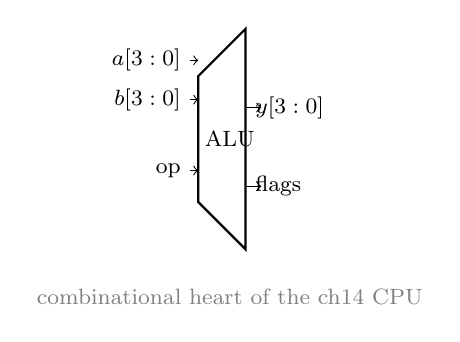
\begin{tikzpicture}[font=\footnotesize]
\draw[thick] (0,0) -- (0,1.6) -- (0.6,2.2) -- (0.6,-0.6) -- cycle;
\node at (0.4,0.8) {ALU};
\node[left] at (-0.1,1.8) {$a[3:0]$}; \draw[->] (-0.1,1.8) -- (0,1.8);
\node[left] at (-0.1,1.3) {$b[3:0]$}; \draw[->] (-0.1,1.3) -- (0,1.3);
\node[left] at (-0.1,0.4) {op}; \draw[->] (-0.1,0.4) -- (0,0.4);
\node[right] at (0.6,1.2) {$y[3:0]$}; \draw[->] (0.6,1.2) -- (0.8,1.2);
\node[right] at (0.6,0.2) {flags}; \draw[->] (0.6,0.2) -- (0.8,0.2);
\node[gray] at (0.4,-1.2) {combinational heart of the ch14 CPU};
\end{tikzpicture}

\caption{The ALU as a symbol. Notice it is pure combination: data in,
result out — no memory. The \texttt{flags} output is just comparators'
results bundled out for later chapters to use.}
\label{fig:alu}
\end{figure}

\section{Common mistakes}
\label{sec:mistakes09}

\begin{itemize}
\item \textbf{K-map adjacency slips}: the edges wrap — top touches
bottom, left touches right. A group of 4 that is not a rectangle is not
a group.
\item \textbf{Incomplete truth tables}: a missing row is not a 0; feed
the minimizer all $2^n$ rows or it will ``minimize'' a lie.
\item \textbf{Treating don't-cares as values}: \texttt{x} means
``whatever is cheapest,'' not ``0'' — if the input can actually occur,
it was never a don't-care.
\item \textbf{Forgetting \texttt{default}} in a \texttt{case}: unlisted
rows leave wires undriven and synthesize latches, not logic.
\item \textbf{Confusing encoder and decoder direction}: decoder spreads
one code to many lines; encoder packs many lines to one code.
\end{itemize}

\section{Exercises}
\label{sec:exercises09}

\begin{exercise}[easy]
Write the 4:1 mux truth table for $d_0..d_3$ and $s_1s_0$; how many rows?
\end{exercise}
\begin{exercise}[easy]
Half-adder: show $s=a\oplus b$ and $c=ab$ from the truth table.
\end{exercise}
\begin{exercise}[easy]
What does a 3-to-8 decoder output when $s=101$, $e=1$? When $e=0$?
\end{exercise}
\begin{exercise}[easy]
In our ripple chain, why does $c_4$'s delay not depend on the data
pattern? When does it?
\end{exercise}
\begin{exercise}[medium]
Design a 4:2 priority encoder: inputs $i_0..i_3$ (highest first),
output the index of the highest asserted bit plus a valid flag. Write
the truth table using don't-cares.
\end{exercise}
\begin{exercise}[medium]
Show a subtractor is ``an adder plus two's complement'': write
$y=a-b$ as $a+\bar b+1$ in gates, reusing the adder4 structure.
\end{exercise}
\begin{exercise}[medium]
Estimate how many LUTs (a 4-input truth table each) a function of 6
inputs needs in the worst case, and how many if it factors neatly.
\end{exercise}
\begin{exercise}[medium]
Seven-seg segment $e$ is on for digits $\{0,2,6,8\}$. Using rows 10--15
as don't-cares, minimize $e$ on paper.
\end{exercise}
\begin{exercise}[hard]
(Implement) Extend \texttt{ch09\_adder4\_tb.v} to drive all $16^2$ pairs
and assert \texttt{cout,sum == a+b} each row; run it and report.
\end{exercise}
\begin{exercise}[hard]
A comparator: write the 2-bit-magnitude comparison $a>b$ as a Boolean
expression, then show it equals ``subtract and check the borrow.''
\end{exercise}

\section{Summary}
\label{sec:summary09}

\begin{center}\small
\begin{tabular}{@{}p{0.30\linewidth}p{0.62\linewidth}@{}}
\toprule
\textbf{Block} & \textbf{One-line version} \\ \midrule
Mux & Data selects which input passes; decoder's dual. \\
Decoder & One enable, $2^n$ mutually-exclusive lines. \\
Half / full adder & XOR+AND, then XOR chain + carry-merge; the cell. \\
Ripple carry & $n$ FAs chained; worst delay $\sim 2n$ levels. \\
Two-level carry & $\sim$4 levels but $2^n$ terms — speed bought with area. \\
Comparator & A subtractor read for sign only. \\
Priority encoder & ``First wins'': \texttt{casez} + don't-cares. \\
Seven-seg decoder & Seven 4-input functions sharing one truth table. \\
ALU & Mux + adder + comparator = the combinational CPU heart. \\
\bottomrule
\end{tabular}
\end{center}

\section*{Notes}
\begin{enumerate}
\item Harris \& Harris, \emph{Digital Design and Computer Architecture},
ch.\ 2, 5 — mux/decoder structure, adder taxonomy~\cite{ddca}.
\item \emph{All About Circuits}, Vol.~IV: Digital — combinational
building blocks~\cite{aacvol4}.
\item \emph{fpga4fun.com} — small complete FPGA projects, the book's
``one project per concept'' model~\cite{fpga4fun}.
\end{enumerate}

\section*{Hints and answers}
\begin{description}
\item[2:1 mux (easy)] $y=\bar s d_0 + s d_1$ — decoder of $s$ feeding
ANDs into an OR, the universal 2-level shape.
\item[16-bit delay (medium)] $\approx 2n=32$ levels ripple vs
$\sim 2^{16}$ terms for a flat $c_{16}$ — the trade explodes, so lookahead
splits the difference.
\item[Default policy (medium)] \texttt{1010} $\to$ \texttt{0000000} —
dark. A minimizer using the \texttt{x} rows could legally show
anything; it owes correctness only on rows 0--9.
\item[4:1 table (easy)] 4 select states $\times$ don't-care data = 16
rows enumerated.
\item[Half adder (easy)] $s=1$ iff $a\ne b$; $c=1$ iff $a=b=1$.
\item[Decoder (easy)] $s=101,e=1$: line 5 high; $e=0$: all zero.
\item[Ripple delay (easy)] Worst case is data-independent (carry must
propagate end-to-end); average case depends on the operands.
\item[Priority encoder (medium)] Rows like \texttt{1---} $\to$ index 0
when $i_0=1$ regardless of the rest.
\item[Subtractor (medium)] Invert $b$, set $c_0=1$: one inverter row
plus the same chain — the adder computes $a+(\bar b+1)$.
\item[LUTs (medium)] Naive $2^6=64$ rows on 4-input LUTs; a factored
function can be a handful — structure matters more than input count.
\item[Segment $e$ (medium)] $e = \bar d_0\,(\bar d_2 + d_1)$ — two
groups of four, exploiting three \texttt{x} cells.
\item[Exhaustive tb (hard)] Loop \texttt{a} 0--15, \texttt{b} 0--15,
compare \texttt{\{cout,sum\}} to \texttt{a+b}; 256 rows, all pass.
\item[Comparator (hard)] $a>b$: $a_1\bar b_1 +
(a_1 \odot b_1)\,a_0\bar b_0$ with $\odot$ XNOR — equivalently, the
borrow out of $a-b$.
\end{description}
